\section{Serverside}
\begin{frame}{Indledende Id�}
	\begin{block}{Arbejdsark}
		\centering
		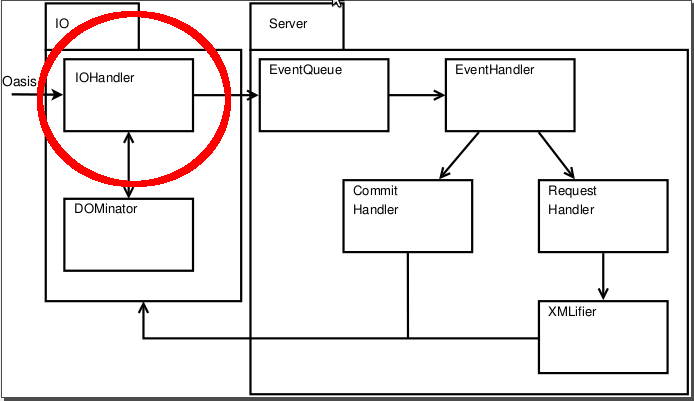
\includegraphics[width=1.00\textwidth]{Img/iniio.png}
	\end{block}
\end{frame}

\section{- Solution}
\begin{frame}[fragile]{Input Handling}
	\begin{block}{Transmissions}
		\begin{lstlisting}[keywordstyle=\color{black}]
			Ping: TYPE[int]PING[size]="randomBytes"
			 int  = int, CRUD value
			 size = int, how many random bytes
			 
			Request: TYPE[int1]MXML[length,int2]="xmlData"[ACCEPT]
			 int1    = int, CRUD value
			 length  = int, length of xmlData
			 int2    = boolean, more files comming ? False for Request
			 
			COMMIT: TYPE[int1]MXML[length,int2]="xmlData"
			            FILE[length2,name.ext,int3]="fileData"[ACCEPT]
			 int1     = int, CRUD value
			 length   = int, length of xmlData
			 int2     = boolean, any files comming ? False if no file(s)
			 length2  = long, size of file
			 name.ext = String, name and extension of file
			 int3     = boolean, more files comming ?
		\end{lstlisting}
	\end{block}
\end{frame}

\begin{frame}{Input Handling}
	\begin{block}{Ping}
		\begin{figure}
			\centering
			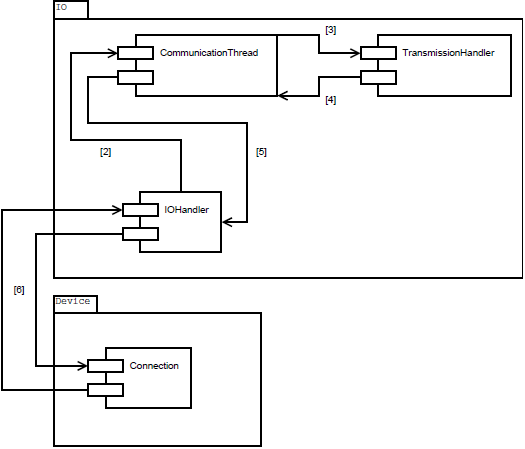
\includegraphics[width=0.85\textwidth]{Img/ping.png}
			\label{fig:ping}
		\end{figure}
	\end{block}
\end{frame}

\begin{frame}{Input Handling}
	\begin{block}{Commit and Request}
		\begin{figure}
			\centering
			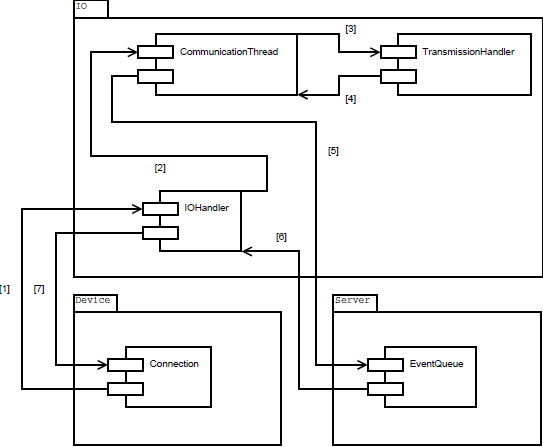
\includegraphics[width=0.85\textwidth]{Img/requestCommit.png}
			\label{fig:requstCommit}
		\end{figure}
	\end{block}
\end{frame}


\begin{frame}
 \begin{block}{Arbejdsark}
  \begin{figure}
   \centering
   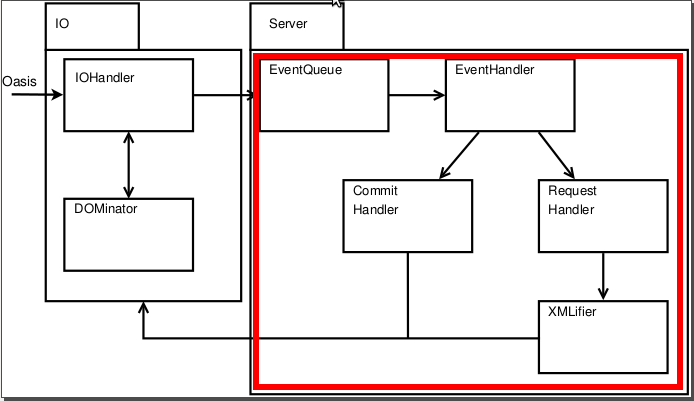
\includegraphics[width=1.00\textwidth]{Img/inixq.png}
  \end{figure}
 \end{block}
\end{frame}


\begin{frame}{XML and Queries}
  \begin{block}{sw6ml}
    \begin{figure}
      \centering
      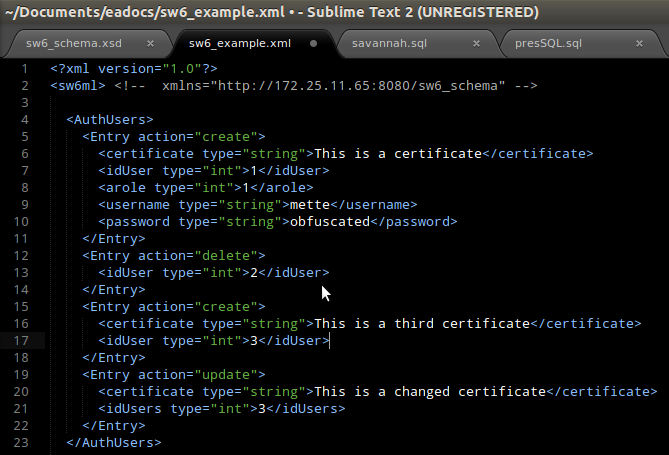
\includegraphics[width=1.00\textwidth]{Img/xml.png}
    \end{figure}

  \end{block}
\end{frame}

\begin{frame}{XML and Queries}
  \begin{block}{Query Handling}
    \begin{figure}
     \centering
     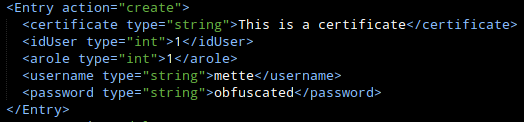
\includegraphics[width=1.00\textwidth]{Img/entry.png}
    \end{figure}
    
    \begin{figure}
      \centering
      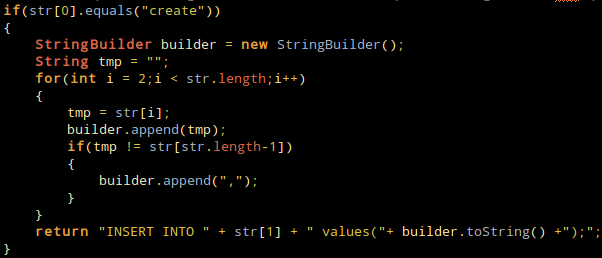
\includegraphics[width=1.00\textwidth]{Img/entryjava.png}
    \end{figure}
   
  \end{block}
\end{frame}

\begin{frame}{XML and Queries}
  \begin{block}{Query Handling Continued}
  INSERT INTO AuthUsers values('this is a certificate',1,1,'mette','obfuscated');
  \end{block}
\end{frame}

\section{ - Test} 
\begin{frame}{Test}
  \begin{block}{Tests}
    48 JUnit test cases  \\
    764 ad hoc test lines  \\
    1 Big bang system test  \\
  \end{block}
\end{frame}

\begin{frame}{Demo}
\end{frame}

\begin{frame}{Scrum}
 \begin{block}{Tilpasset Scrum}
   Standup meetings \\
   XP koncepter - Pair programming \\
   Sprint l�ngde \\
   Kunde involvering \\
   Scrum roller \\
 \end{block}
\end{frame}

\begin{frame}{Konklusion}
 \begin{block}{}
   Vi er igang..\\
   Men ikke f�rdig ..\\
    \pause
   Ang�ende Scrum ..\\
 \end{block}
\end{frame}






